\chapter{Diagramme de classes}
Les documents XML bien formés répondront à l'arborescence présentée ci-dessous.

Les hypothèse suivantes sont également formulées :
\begin{itemize}
    \item Les documents XML à parser ne contiendront pas de DTD interne
    \item Les Process Instruction (PI) ne contiendront que des attributs
    \item Aucune référence ne sera présente dans les documents XML\\
\end{itemize}

Les classes ici décrites seront rattachées au namespace "Xml" défini en C++.

\section{Document}
Cette classe contient un prolog, un élément racine de type Element et un ensemble de fils de type DocumentNode (liste pouvant contenir 0 à N éléments).

\section{MiscNode}
Cette classe abstraite permet à la classe Document de contenir 0 à N éléments Misc.
    On notera ici qu'une relation de spécialisation représente le symbole $'|'$ (alternative) dans une règle BNF.

\section{Comment}
Contient la description d'un commentaire sous forme de chaîne de caractères.

\section{Processing Instruction}
En accord avec l'hypothèse énoncée précédemment, une PI ne contient qu'un nom et une liste ordonnée d'attributs

\section{Attribute}
Cette classe décrit un attribut sous la forme suivante
mName = "mValue"

\section{DocumentNode}
Une instance de cette classe peut être de type Element, Text Comment ou PI. Afin de garantir la cohérence de l'architecture XML, ce noeud dispose d'un pointeur sur son noeud parent.

\section{Element}
Un élément XML dispose d'un nom de balise, d'un ensemble ordonné d'attributs et d'un ensemble ordonné de noeuds fils. Cet élément peut être une balise vide ($<br/>$).

\section{Text}
Un noeud texte est naturellement décrit par une chaîne de caractères. Celui-ci ne dérive pas de la classe MiscNode puisque, si son contenu s'apparente à celui d'un noeud Comment, il ne peut en revanche être contenu par une instance de Document. Il est alors nécessaire d'ajouter un niveau de spécialisation afin d'éviter une relation incohérente.

\section{ElementIterator}
Cet élément est dédié au parcours de l'arbre XML, de manière similaire à un parseur de type SAX.

\begin{landscape}
\begin{figure}[h!]
    \centering
    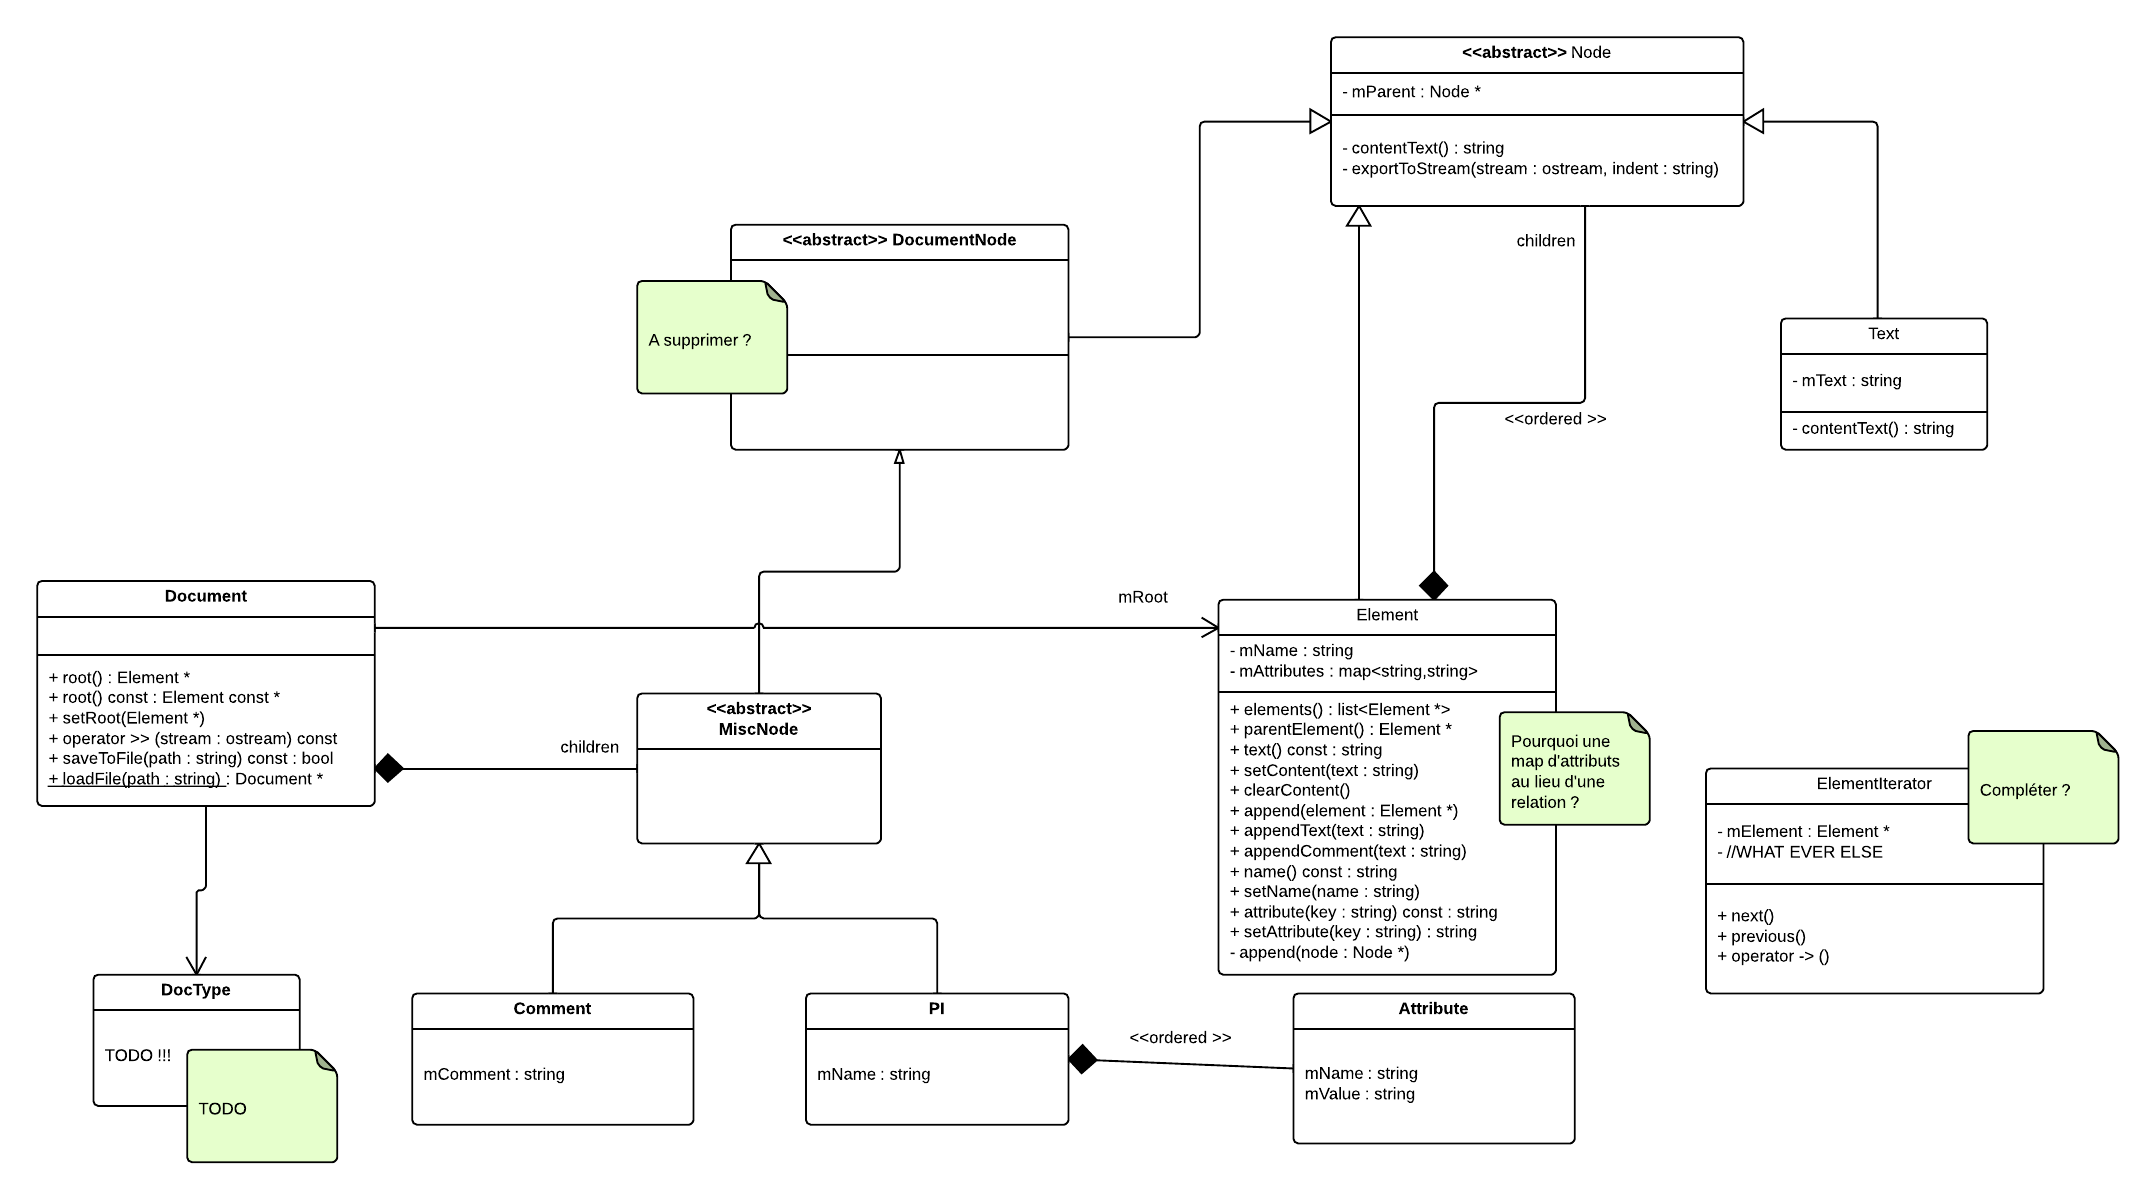
\includegraphics[width=\linewidth]{images/classDiagram.png}
    \caption{Diagramme de classes de l'arborescence XML}
    \label{classDiagram}
\end{figure}
\end{landscape}
